\documentclass[conference]{IEEEtran}

\usepackage[T1]{fontenc}
\usepackage[table]{xcolor}
\usepackage{graphicx}
\usepackage{booktabs}
\usepackage{amsmath,amssymb}
\usepackage{tikz}
\usetikzlibrary{arrows.meta,positioning,shapes.geometric}
\usepackage{listings}
\usepackage{url}
\usepackage{cite}
\usepackage{hyperref}
\usepackage{balance}

\definecolor{docintelNavy}{HTML}{173B63}
\definecolor{docintelBlue}{HTML}{2F75B5}
\definecolor{docintelLightBlue}{HTML}{DCEBFA}
\definecolor{docintelPaleBlue}{HTML}{F1F7FC}
\hypersetup{colorlinks=true,linkcolor=docintelNavy,citecolor=docintelNavy,urlcolor=docintelBlue}
\definecolor{codegray}{gray}{0.95}
\lstset{basicstyle=\ttfamily\footnotesize,backgroundcolor=\color{docintelPaleBlue},rulecolor=\color{docintelBlue},
        breaklines=true,frame=single,captionpos=b,columns=fullflexible}

\title{DocIntel: A Provider-Flexible, Privacy-Oriented Document Intelligence Workspace\\
\large System Design, Implementation, and Evaluation}

\author{\IEEEauthorblockN{Samar Mittal\IEEEauthorrefmark{1},
Rajkumar Santra\IEEEauthorrefmark{2}, and Sonam Maurya\IEEEauthorrefmark{3}}
}

\begin{document}
\maketitle

\begin{abstract}
Modern document repositories contain heterogeneous content, including text-native files, scanned pages, spreadsheets, tables, URLs, and multimedia sources. This paper presents DocIntel, a containerized document-intelligence workspace that combines document extraction, optional layout-aware optical character recognition (OCR), vector retrieval, provider-selectable generative models, notebook-oriented conversation, and downloadable visual explanations. The system separates the browser interface, API, processing workers, model providers, and persistent storage, while allowing deployments to use local or cloud AI providers. The implementation is described in terms of Next.js, FastAPI, LangGraph/LangChain orchestration, SurrealDB, and optional Docling processing. This paper documents the architecture, retrieval workflow, privacy and security boundaries, implementation methodology, reproducibility procedure, and validation evidence reported for the project. A preliminary evaluation of nine synthetic railway-domain documents observed successful extraction for three PDF, three DOCX, and three XLSX files; backend visualization tests and frontend component tests also passed in the reported development snapshot. OCR-quality claims are scoped separately because the initial text-native sample corpus does not establish scanned-document accuracy.
\end{abstract}

\begin{IEEEkeywords}
Document intelligence, retrieval-augmented generation, OCR, vector search, knowledge workspace, multilingual interfaces, document layout analysis, provider interoperability
\end{IEEEkeywords}

\section{Introduction}
Organizations and researchers increasingly work with large, heterogeneous collections of documents. Conventional repositories support storage and keyword search but provide limited support for source-grounded question answering, cross-document synthesis, visual reasoning, or structured transformation. Information can also be lost when a document contains scans, complex tables, figures, formulas, or multiple reading orders. Retrieval-augmented generation (RAG) addresses part of this problem by retrieving evidence before language-model generation, but a useful workspace must also preserve source provenance, user control, persistent research context, and deployment flexibility \cite{lewis2020rag}.

DocIntel is presented as a private research workspace built around a user-managed collection of sources. A source may be a document, URL, text, audio, video, or supported image. The application extracts content, optionally performs OCR and layout analysis, prepares retrieval context, and supports notebook chat, source chat, transformations, summaries, and generated visualizations. Its design permits interchangeable cloud or local language and embedding models rather than binding every workflow to one vendor \cite{docintel}.

\subsection{Research Objectives}
The principal objectives are:
\begin{enumerate}
  \item integrate heterogeneous source ingestion and document extraction into one workflow;
  \item support layout-aware OCR without making it mandatory for lightweight deployments;
  \item provide source-grounded retrieval with configurable embedding and chat models;
  \item separate application logic, persistent storage, and external AI providers;
  \item support reproducible local deployment through Docker Compose; and
  \item provide visual explanations through Mermaid and Matplotlib.
\end{enumerate}

\subsection{Research Questions}
\begin{itemize}
  \item \textbf{RQ1:} How can heterogeneous document sources be processed through one extensible pipeline?
  \item \textbf{RQ2:} What architectural choices permit cloud and local models without vendor lock-in?
  \item \textbf{RQ3:} How does optional OCR change extraction behavior for scanned and complex documents?
  \item \textbf{RQ4:} Which deployment, retrieval, privacy, and reproducibility properties should a research document workspace guarantee?
  \item \textbf{RQ5:} Which implementation-level security controls are necessary when generating visual output?
\end{itemize}

\section{Related Work and Positioning}
Document intelligence combines OCR, document-layout analysis, information extraction, semantic retrieval, and generative language models. Classical OCR systems recognize characters but may not preserve reading order, section hierarchy, captions, tables, and document-level structure. Layout-aware systems can reduce these losses by representing page structure and content objects. Tesseract is a widely used OCR engine, while Docling provides a document-conversion and layout-processing framework \cite{smith2007tesseract,docling}.

RAG retrieves relevant contextual evidence before an answer is generated \cite{lewis2020rag}. Vector embeddings map semantically related text into a shared representation space, enabling similarity search beyond exact keyword matches. Retrieval quality therefore depends on extraction quality, chunking strategy, embedding-model selection, retrieval parameters, and generation behavior. DocIntel separates these choices so that chat and embedding models need not come from the same provider \cite{docintel}.

\begin{table}[!t]
\centering
\caption{Architectural comparison with document-processing alternatives}
\label{tab:positioning}
\small
\setlength{\tabcolsep}{2pt}
\begin{tabular}{p{0.18\columnwidth}p{0.34\columnwidth}p{0.40\columnwidth}}
\toprule
\rowcolor{docintelLightBlue}
Approach & Strength & Limitation \\
\midrule
Tesseract OCR & Mature and local; broad script support & Layout and language configuration may require additional integration \\
PaddleOCR \cite{paddleocr} & Flexible detection and recognition pipelines & RAG, notebooks, and application state require separate integration \\
Cloud document APIs & Managed layout/OCR and scaling & Vendor dependency, network transfer, usage charges, and regional/privacy constraints \\
DocIntel & Integrated ingestion, OCR option, notebooks, retrieval, and provider control & Requires evaluation of each selected extraction stack and external services for most cloud models \\
\bottomrule
\end{tabular}
\end{table}

Table~\ref{tab:positioning} is an architectural comparison, not a benchmark conclusion. A defensible performance comparison requires a common document corpus, OCR metrics, cost measurements, and controlled model configurations.

\section{System Architecture}
DocIntel is deployed with Docker Compose as two primary services: the application and SurrealDB. The application image contains the Next.js frontend, FastAPI API, background processing runtime, and AI workflows. SurrealDB stores persistent application records, processing state, credential metadata, and vectors. User files and runtime state are stored in the notebook data volume \cite{docintel,surrealdb}.

\begin{figure*}[!t]
\centering
\resizebox{\textwidth}{!}{%
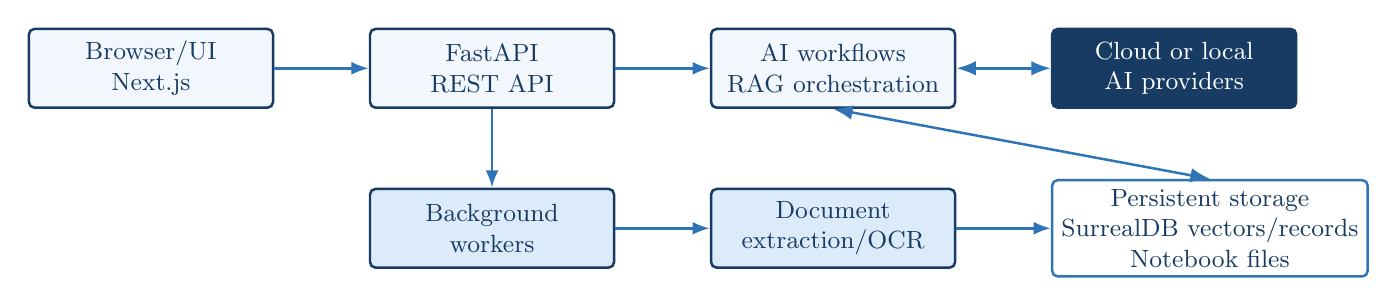
\begin{tikzpicture}[node distance=10mm and 12mm,
  component/.style={draw=docintelNavy,fill=docintelPaleBlue,text=docintelNavy,rounded corners=2pt,align=center,minimum height=10mm,minimum width=31mm,font=\small,line width=0.9pt},
  process/.style={component,fill=docintelLightBlue},
  store/.style={component,fill=white,draw=docintelBlue},
  provider/.style={component,fill=docintelNavy,text=white},
  flow/.style={-{Latex[length=2.2mm]},draw=docintelBlue,line width=0.9pt},
  exchange/.style={<->,>=Latex,draw=docintelBlue,line width=0.9pt}]
\node[component] (browser) {Browser/UI\\Next.js};
\node[component,right=of browser] (api) {FastAPI\\REST API};
\node[component,right=of api] (graphs) {AI workflows\\RAG orchestration};
\node[provider,right=of graphs] (providers) {Cloud or local\\AI providers};
\node[process,below=of api] (worker) {Background\\workers};
\node[process,right=of worker] (extract) {Document\\extraction/OCR};
\node[store,right=of extract] (storage) {Persistent storage\\SurrealDB vectors/records\\Notebook files};
\draw[flow] (browser)--(api);
\draw[flow] (api)--(graphs);
\draw[exchange] (graphs)--(providers);
\draw[flow] (api)--(worker);
\draw[flow] (worker)--(extract);
\draw[flow] (extract)--(storage);
\draw[exchange] (graphs.south)--(storage.north);
\end{tikzpicture}%
}
\caption{DocIntel runtime architecture. Blue arrows indicate processing or data exchange.}
\label{fig:architecture}
\end{figure*}


\subsection{Frontend}
The Next.js frontend provides notebooks, sources, settings, search, chat, Markdown, podcast controls, and visualization rendering. The interface uses browser-language detection, a saved preference, and an English fallback. Selecting an interface locale does not itself translate source text; translation or multilingual understanding depends on a configured language or embedding model when appropriate \cite{docintel}.

\subsection{API and Background Processing}
FastAPI is responsible for authentication, provider credentials, model configuration, source creation, notebook operations, chat, transformations, search, jobs, and visualization endpoints. Long-running extraction, embedding generation, transformation, and podcast jobs are delegated through a worker/runtime path so that requests can be processed asynchronously. Processing status should be checked through the API or user interface rather than assumed complete after upload \cite{docintel}.

\subsection{AI Orchestration}
LangGraph/LangChain-oriented workflows assemble prompts and source context, invoke a configured provider, and stream output. Chat and embeddings can be configured independently. This separation permits a local embedding model with a cloud language model, or both remote, local, or mixed according to latency, cost, and privacy requirements \cite{langgraph,docintel}.

\subsection{Storage and Persistence}
SurrealDB stores notebooks, sources, notes, processing state, credential metadata, jobs, and vector records. Uploaded source files and caches are under \texttt{notebook\_data}; database state is under \texttt{surreal\_data}. These volume semantics are important for backup, migration, and data-retention policy \cite{docintel,surrealdb}.

\section{Document Processing Pipeline}
\begin{figure*}[!t]
\centering
\resizebox{\textwidth}{!}{%
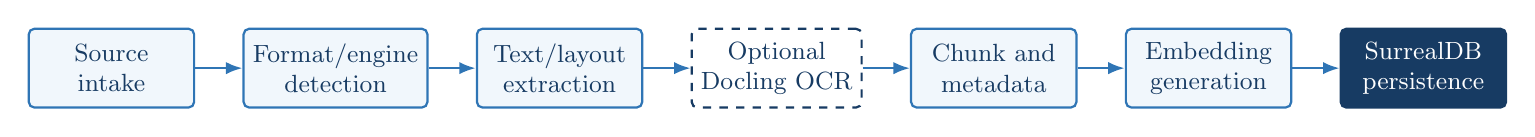
\begin{tikzpicture}[node distance=6mm,
  stage/.style={draw=docintelBlue,fill=docintelPaleBlue,text=docintelNavy,rounded corners=2pt,align=center,font=\small,minimum width=21mm,minimum height=10mm,line width=0.8pt},
  optional/.style={stage,draw=docintelNavy,fill=white,dashed},
  storage/.style={stage,draw=docintelNavy,fill=docintelNavy,text=white},
  flow/.style={-{Latex[length=2.1mm]},draw=docintelBlue,line width=0.9pt}]
\node[stage] (upload) {Source\\intake};
\node[stage,right=of upload] (detect) {Format/engine\\detection};
\node[stage,right=of detect] (extract) {Text/layout\\extraction};
\node[optional,right=of extract] (ocr) {Optional\\Docling OCR};
\node[stage,right=of ocr] (chunk) {Chunk and\\metadata};
\node[stage,right=of chunk] (embed) {Embedding\\generation};
\node[storage,right=of embed] (store) {SurrealDB\\persistence};
\draw[flow] (upload)--(detect);
\draw[flow] (detect)--(extract);
\draw[flow] (extract)--(ocr);
\draw[flow] (ocr)--(chunk);
\draw[flow] (chunk)--(embed);
\draw[flow] (embed)--(store);
\end{tikzpicture}%
}
\caption{Source processing and retrieval-preparation pipeline; OCR is optional.}
\label{fig:pipeline}
\end{figure*}


\subsection{Source Ingestion}
Supported sources are normalized into application content and metadata. Files include text-bearing formats such as PDF, DOCX, and XLSX, while URLs, text, audio, and video use their respective content handlers. Format-specific extraction should preserve source identifiers so that responses can refer to original source records and retrieved evidence \cite{docintel}.

\subsection{Extraction and OCR}
DocIntel uses content-core extraction as the baseline and may enable Docling as an optional runtime. When enabled, Docling can perform layout-aware processing, OCR, table extraction, formula recognition, reading-order analysis, and image-oriented processing. OCR must be evaluated separately from native-text extraction: a text-native PDF may bypass OCR regardless of image quality, and extraction settings can change the output \cite{docling}.

\subsection{Retrieval and Generation}
Extracted text is segmented into chunks and associated with source metadata. The embedding provider generates vector representations stored by the application. A retrieval request searches for relevant vectors and metadata, assembles context, and invokes a selected language model. The model may also rely on notebook instructions, source instructions, conversation state, and transformation prompts \cite{docintel}.

The conceptual workflow is
\begin{equation}
 R(q)=\operatorname{TopK}_{c \in C}\left(\cos(E_q(q),E_c(c))\right),
\end{equation}
where $q$ is the query, $C$ is the source corpus, $E_q$ and $E_c$ are embedding functions, and the top-$K$ contexts are passed to generation. If the embedding model changes, vectors from different models should not be mixed. Existing sources generally require re-embedding for retrieval consistency.

\section{Visual Explanation and Multimodal Features}
DocIntel can render Mermaid diagrams as SVG blocks and generate Matplotlib/Python visualizations. It also supports conversion to TikZ/PGFPlots where applicable and allows generated SVG and source downloads. Mermaid uses strict rendering and SVG sanitization. Python plotting applies abstract-syntax-tree validation, restricted imports, private-attribute restrictions, timeouts, output limits, temporary working directories, and process controls. These controls reduce risk but do not constitute an untrusted-code sandbox suitable for public tenants \cite{docintel}.

The visualization capability should be considered generated presentation logic rather than ground-truth analysis. Numerical claims should be calculated reproducibly and checked against source evidence.

\section{Provider Configuration}
DocIntel supports provider credentials for cloud and local systems, including OpenAI-compatible providers and Ollama. The provider registry determines required credentials and supported modalities. Model categories include language/chat, embedding, speech-to-text, and text-to-speech. Chat models must not be treated as embedding models unless the provider explicitly supports an embedding modality \cite{docintel,ollama}.

Google Gemini Embedding 001 is an embedding option when the Google provider credential is configured. Newer or multimodal embedding models should be used only after confirming compatibility with the installed DocIntel/provider contract. Embedding dimensions and provider compatibility affect model migration; changing embeddings requires re-processing existing sources \cite{googleembed}.

As an offline option, Ollama can host models such as \texttt{nomic-embed-text}. For Docker deployment, the host may need to be addressed as \texttt{host.docker.internal}; this differs between operating systems and firewall configurations \cite{ollama}.

\section{Deployment Methodology}
DocIntel uses a persistent Docker deployment. A typical setup is:
\begin{lstlisting}[language=bash,caption={Deployment commands}]
cp .env.example .env
openssl rand -hex 32
# Configure OPEN_NOTEBOOK_ENCRYPTION_KEY in .env
docker compose up -d --build
docker compose ps
docker compose logs -f open_notebook
\end{lstlisting}

The default user-facing ports are 8502 for the Next.js interface and 5055 for the API. SurrealDB is bound locally in the documented deployment. Stable encryption keys are required: replacing the key can make existing encrypted credentials unreadable. Provider credentials should be configured through the UI and not committed to version control \cite{docintel}.

\section{Security and Privacy}
DocIntel exposes several important privacy boundaries. Provider credentials are encrypted with a configured application key. Application files and runtime state persist separately from SurrealDB. Public repositories should exclude \texttt{.env}, uploads, databases, API keys, notebooks, caches, and generated runtime state. Cloud providers receive source context when their model is selected and queried \cite{docintel}.

Additional controls include strict Mermaid rendering, SVG sanitization, restricted Python execution, host/port isolation, and configurable authentication or password protection. A public deployment should also add HTTPS, authenticated administrative routes, database access controls, source-size limits, rate limiting, audit logging, backup policies, and isolated execution for untrusted visualizations. These recommendations do not imply that every control is currently implemented.

\section{Evaluation}
\subsection{Implementation Validation}
The repository has separate backend visualization tests and frontend test suites. The development snapshot reported during project work included seven backend visualization tests and 182 frontend tests across 35 files. The frontend production build and Docker Compose configuration were also reported as validated. These are author-reported snapshots, not independently reproduced results, and should be regenerated with the software version used for publication \cite{docintel}.

\subsection{Text-Native Extraction Study}
A small synthetic railway-domain corpus containing three PDF, three DOCX, and three XLSX documents was used to test ingestion. All nine files were reported successfully extracted. This establishes format compatibility and persistence through a representative processing path, not OCR effectiveness or end-to-end retrieval correctness.

\begin{table}[!t]
\centering
\caption{Text-native extraction validation reported for the synthetic corpus}
\label{tab:extract}
\small
\begin{tabular}{lccc}
\toprule
\rowcolor{docintelLightBlue}
Format & Files & Successful & Result \\
\midrule
PDF & 3 & 3 & Native text/tables processed \\
DOCX & 3 & 3 & Document text processed \\
XLSX & 3 & 3 & Spreadsheet content processed \\
\midrule
Total & 9 & 9 & 100\% reported success \\
\bottomrule
\end{tabular}
\end{table}

\subsection{Recommended OCR Evaluation}
Because OCR accuracy cannot be inferred from native-format extraction, publication-grade evaluation should use a corpus with known ground truth. Suggested metrics include character error rate (CER), word error rate (WER), table-cell accuracy, reading-order similarity, and formula-recognition accuracy. Evaluation should report per-language and per-document-type results and include:
\begin{itemize}
 \item low-resolution scans;
 \item skew and rotation;
 \item shadows and uneven illumination;
 \item multi-column pages;
 \item handwritten and mixed-language text;
 \item embedded tables, formulas, captions, and stamps; and
 \item native PDF, scanned PDF, and image comparisons.
\end{itemize}

\subsection{Recommended Retrieval Evaluation}
A reusable retrieval benchmark should contain verified questions, source citations, and expected passages. Recommended metrics are Recall@$K$, Mean Reciprocal Rank, NDCG, answer faithfulness, citation support, and human preference. Experiments should compare at least:
\begin{enumerate}
 \item native extraction with no OCR;
 \item Docling/OCR-enabled extraction;
 \item Google Gemini Embedding 001;
 \item a local Ollama embedding model; and
 \item multiple chunk sizes and top-$K$ retrieval depths.
\end{enumerate}

\subsection{Comparative Evaluation of Open-Source Models Through Ollama}
Provider flexibility permits controlled comparison of open-source language models without changing the DocIntel processing or retrieval implementation. Ollama can expose local models through a provider endpoint, allowing the same extracted corpus, chunks, retrieval configuration, prompts, and questions to be tested across models. This comparison evaluates generation behavior, not the Ollama runtime alone.

The primary comparison should record model family, parameter count, quantization, Ollama tag, context length, hardware, temperature, and inference time. Candidate models should be selected according to available memory and document-language requirements. Models must be treated as configurations rather than interchangeable versions: changing quantization or model revision is an experimental condition that must be recorded.

A recommended open-model study follows the same fixed RAG pipeline for each model:
\begin{enumerate}
 \item select one embedding model for all runs;
 \item process one fixed document corpus with identical extraction and chunking settings;
 \item use the same retrieval depth and identical prompts;
 \item generate answers to questions with verified supporting passages;
 \item repeat each condition sufficiently to report variance; and
 \item record model load time, first-token latency, end-to-end latency, throughput, memory, and available energy measurements.
\end{enumerate}

\begin{table}[!t]
\centering
\caption{Suggested open-model comparison design}
\label{tab:modelcomparison}
\scriptsize
\begin{tabular}{p{1.65cm}p{2.05cm}p{3.45cm}}
\toprule
\rowcolor{docintelLightBlue}
Dimension & Controlled setting & Recorded evidence \\
\midrule
Model & Ollama tag and revision & Parameters, quantization, revision \\
Hardware & Same host for all candidates & CPU/GPU, VRAM, RAM, OS \\
Corpus & Fixed checksummed source set & Pages, languages, question IDs \\
Extraction & Same engine and OCR settings & Extracted text revision \\
Embeddings & One fixed embedding model & Vector revision and dimensions \\
Retrieval & Same chunk size and top-$K$ & Passage IDs and ranks \\
Generation & Same prompt and decoding settings & Answer, tokens, latency, cost \\
Evaluation & Identical scoring procedure & Faithfulness, citations, accuracy, preference \\
\bottomrule
\end{tabular}
\end{table}

Table~\ref{tab:modelcomparison} treats language-generation models as experimental variables. Cloud providers and locally hosted open models should be compared under separate privacy and cost assumptions. A model that cannot fit in memory or cannot complete the context should be reported as a deployment failure rather than assigned a zero answer-quality score without interpretation.

Quality metrics include normalized answer accuracy for closed questions, passage-level Recall@$K$ and MRR for retrieval, answer faithfulness, unsupported-claim rate, citation precision and recall, source-localization accuracy, human preference, latency, throughput, and resource consumption. BLEU or ROUGE can supplement controlled text-generation tasks, while human judgments should remain primary for synthesized research answers. API charges are not the only cost: local inference consumes hardware, electricity, maintenance, and operator time. Numerical results should not be reported until controlled experiments under the same conditions have been completed.

\section{Reproducibility and Experimental Protocol}
\begin{enumerate}
 \item Start from a clean commit and record its hash, image identifiers, dependency lockfiles, Ollama version, and model tags.
 \item Configure a stable encryption key and keep provider credentials outside version control.
 \item Import a fixed corpus and retain its checksums.
 \item Record extraction-engine, OCR, chunking, embedding, language-model, temperature, and retrieval settings.
 \item Run source processing and wait for completion status.
 \item Export extracted text and metadata without exposing private source content.
 \item Execute retrieval and answer-generation queries using a fixed seed when supported.
 \item Record provider, latency, cost, token usage, and generated answer.
 \item Compare only runs that use compatible embedding spaces.
 \item Rebuild embeddings after changing embedding providers or models.
 \item Perform human verification for provenance and factual faithfulness.
 \item Publish commands, configuration templates, aggregate metrics, failed cases, and environment limitations.
\end{enumerate}

A reproducible result must distinguish software compatibility from model quality. Container health, successful processing, and API connectivity do not establish answer correctness.

\section{Threats to Validity}
\begin{itemize}
 \item \textbf{Corpus bias:} The existing railway corpus is small and synthetic.
 \item \textbf{OCR bias:} Native-format extraction does not measure OCR.
 \item \textbf{Provider drift:} Cloud model behavior, prices, quotas, and identifiers can change.
 \item \textbf{Embedding non-comparability:} Vectors from different models cannot be compared directly.
 \item \textbf{Metric instability:} Automatically generated answers require citation and faithfulness verification.
 \item \textbf{Prompt sensitivity:} Retrieval and generation can vary with instructions and temperature.
 \item \textbf{Privacy leaks:} Shared prompts may transmit source text to configured cloud providers.
 \item \textbf{Localization coverage:} Interface translation is not equivalent to faithful multilingual content understanding.
\end{itemize}

\section{Limitations and Future Work}
Future work should include larger multi-domain OCR benchmarks; systematic table and formula datasets; citation-level evidence evaluation; adversarial source tests; provenance visualization; incremental and differential embedding; privacy-preserving local inference; user studies; and stronger tenant isolation for public deployments. Benchmarks should include OCR engines such as Tesseract, PaddleOCR, and Docling under controlled hardware and model configurations.

Additional engineering work includes immutable document snapshots, chunk provenance, field-level confidence, source-change auditing, encrypted backup procedures, and objective evaluation of response latency and token cost. The Python plotting environment should be moved to a stronger isolated service before accepting untrusted third-party code.

\section{Conclusion}
DocIntel presents an integrated architecture for private document research. It combines heterogeneous ingestion, optional layout-aware OCR, configurable embeddings, retrieval, provider-flexible generation, notebooks, multilingual interface support, and downloadable visual explanations. Its architecture is designed to avoid vendor lock-in while keeping storage and credentials under application control.

Initial project-reported testing confirms compatibility with representative text-native PDF, DOCX, and XLSX sources and reports frontend, visualization-backend, and Docker validation. For publishable scientific claims, OCR, embedding, retrieval, and generation require controlled experiments with documented corpora, metrics, baselines, and uncertainty.

\appendices
\section{Configuration Template}
\begin{lstlisting}[caption={Illustrative environment template}]
OPEN_NOTEBOOK_ENCRYPTION_KEY=<generate-a-stable-random-key>
OPEN_NOTEBOOK_ENABLE_DOCLING=true
SURREAL_USER=root
SURREAL_PASSWORD=<choose-a-private-password>
SURREAL_NAMESPACE=open_notebook
SURREAL_DATABASE=open_notebook
\end{lstlisting}

\section{Data and Software Availability}
The project source repository and execution instructions should be published with dependency lockfiles and Docker Compose configuration. API keys, private documents, databases, notebooks, and runtime data must not be included. Synthetic documents may be distributed if cleared for redistribution; private or unpublished source data should be excluded. A reproducible release should identify the software commit, container image digest, Docling version, provider/model identifiers, and test commands.

\balance
\begin{thebibliography}{10}
\bibitem{lewis2020rag}
P. Lewis, E. Perez, A. Piktus, et al., ``Retrieval-Augmented Generation for Knowledge-Intensive NLP Tasks,'' in \emph{Advances in Neural Information Processing Systems}, 2020.

\bibitem{devlin2019bert}
J. Devlin, M.-W. Chang, K. Lee, and K. Toutanova, ``BERT: Pre-training of Deep Bidirectional Transformers for Language Understanding,'' in \emph{Proceedings of NAACL-HLT}, 2019.

\bibitem{smith2007tesseract}
R. Smith, ``An Overview of the Tesseract OCR Engine,'' in \emph{Proceedings of the Ninth International Conference on Document Analysis and Recognition}, 2007.

\bibitem{paddleocr}
PaddleOCR Contributors, ``PaddleOCR: Multilingual OCR Toolkit,'' software repository. [Online]. Available: \url{https://github.com/PaddlePaddle/PaddleOCR}

\bibitem{docling}
Docling Contributors, ``Docling: Document Processing and Conversion,'' software repository. [Online]. Available: \url{https://github.com/docling-project/docling}

\bibitem{surrealdb}
SurrealDB, ``SurrealDB Documentation.'' [Online]. Available: \url{https://surrealdb.com/docs}

\bibitem{langgraph}
LangChain AI, ``LangGraph Documentation.'' [Online]. Available: \url{https://langchain-ai.github.io/langgraph/}

\bibitem{ollama}
Ollama, ``Ollama Documentation.'' [Online]. Available: \url{https://ollama.com}

\bibitem{googleembed}
Google, ``Gemini Embeddings Documentation.'' [Online]. Available: \url{https://ai.google.dev/gemini-api/docs/embeddings}

\bibitem{docintel}
S. Mittal, ``DocIntel: Document Intelligence Workspace,'' GitHub repository. [Online]. Available: \url{https://github.com/Samar23dev/DocIntel}
\end{thebibliography}

\end{document}
